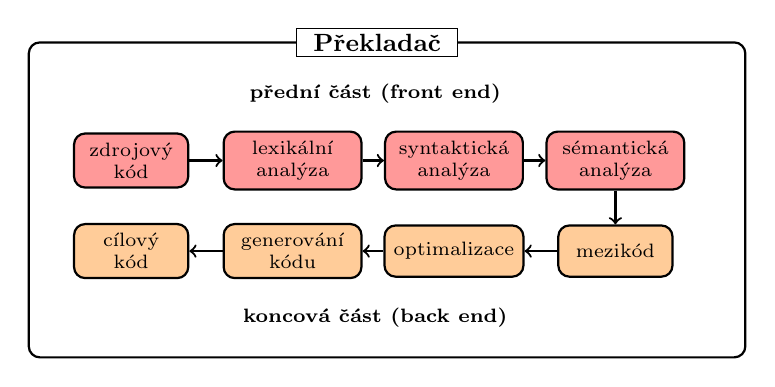
\begin{tikzpicture}[
    phase/.style={
        draw,
        rounded corners,
        thick,
        align=center,
        font=\scriptsize,
        minimum width=1.75cm,
        minimum height=0.65cm
    },
    lang/.style={
        draw,
        rounded corners,
        thick,
        align=center,
        font=\scriptsize,
        minimum width=1.45cm,
        minimum height=0.65cm
    },
    arrow/.style={->, thick}
]
    % vnější obdélník
    \visible<2->{
        \draw[thick, rounded corners] (-1.3,1.5) rectangle (7.8,-2.5);
        \node[draw, fill=white, font=\small\bfseries, inner xsep=6pt, inner ysep=2pt]
            at (3.125,1.5) {Překladač};
    }

    \node<2->[lang,fill=red!40!white]  (src) at (0,0) {zdrojový\\kód};
    \node<3->[phase,fill=red!40!white] (lex) at (2.05,0) {lexikální\\analýza};
    \node<4->[phase,fill=red!40!white] (syn) at (4.10,0) {syntaktická\\analýza};
    \node<5->[phase,fill=red!40!white] (sem) at (6.15,0) {sémantická\\analýza};

    \node<6->[lang,fill=orange!40!white]  (ir)  at (6.15,-1.15) {mezikód};
    \node<7->[phase,fill=orange!40!white] (opt) at (4.10,-1.15) {optimalizace};
    \node<8->[phase,fill=orange!40!white] (gen) at (2.05,-1.15) {generování\\kódu};
    \node<9->[lang,fill=orange!40!white]  (tgt) at (0,-1.15) {cílový\\kód};

    \draw<3->[arrow] (src) -- (lex);
    \draw<4->[arrow] (lex) -- (syn);
    \draw<5->[arrow] (syn) -- (sem);
    \draw<6->[arrow] (sem) -- (ir);
    \draw<7->[arrow] (ir) -- (opt);
    \draw<8->[arrow] (opt) -- (gen);
    \draw<9->[arrow] (gen) -- (tgt);

    \node<5->[font=\scriptsize] at (3.1,0.85) {\textbf{přední část (front end)}};
    \node<8->[font=\scriptsize] at (3.1,-2.0) {\textbf{koncová část (back end)}};

\end{tikzpicture}
